\subsection{Design Choices}
\label{d_choices}

\subsubsection{Model Selection Strategy}
We have mentioned in Section \ref{data} that we match the vehicles with models based on dimension similarity. Now we give the reasons why we choose this strategy. The first reason is that the distribution of models' dimension covers the KITTI vehicles'. Besides, this strategy achieves the best performance among possible strategies as shown in Table \ref{model_selection}. The CAD model dataset provides two sets of dimensions: real-world dimensions and  uniform dimensions where all the width is 1.8 meters. Dims strategy means that the best model is the one whose dimension vector has the least distance to the vehicle's. Dim Ratios strategy is similar but bases on the ratio vector $(height/width, length/width)$ with the uniform dimensions given by the CAD dataset. The rest two are based on Dims and Dim Ratios, \ie using one strategy to select 10 models first and then applying the other to select the best one.

We use two metrics to evaluate these strategies: type accuracy and mean deviation. The types are defined as in Figure \ref{figure:vehicle_dataset}. Vehicle types can present the location of characteristic points of vehicles well because the vehicles' 3D sketches varies a lot among different types but keeps similar with the same type and the dimension variation can be solved via scaling. Therefore we label 1000 KITTI vehicles and test the type matching accuracy among these strategies. The second metric, mean deviation, is the Euclidean distance between the dimension vectors of the selected model and ground truth. Even through the performance of Dims is not that good, it is the best one we can use based on the information provided. Figure \ref{figure:model_selection_s} shows one labelled example where Dims has the most accurate points labelled and the others all label the points around the back wheel wrongly.
\tbd [is it ok to put these bad results here]

\renewcommand{\arraystretch}{1.2}
\begin{table}[ht]
	\centering
	\caption{Performance of four model selection strategies}
	\label{model_selection}
	\resizebox{\textwidth}{!}{
	\begin{tabular}{|c|c|c|c|c|}
		\hline
		& Dim Ratios & Dims  & Dim Ratios \& Dims & Dims \& Dim Ratios \\ \hline
		Type Accuracy      & 0.256      & \textbf{0.463} & 0.137     & 0.160     \\ \hline
		Mean Deviation (m) & 0.631      & \textbf{0.384} & 0.865     & 0.893     \\ \hline
	\end{tabular}
}
\end{table}


\begin{figure}[h]		
	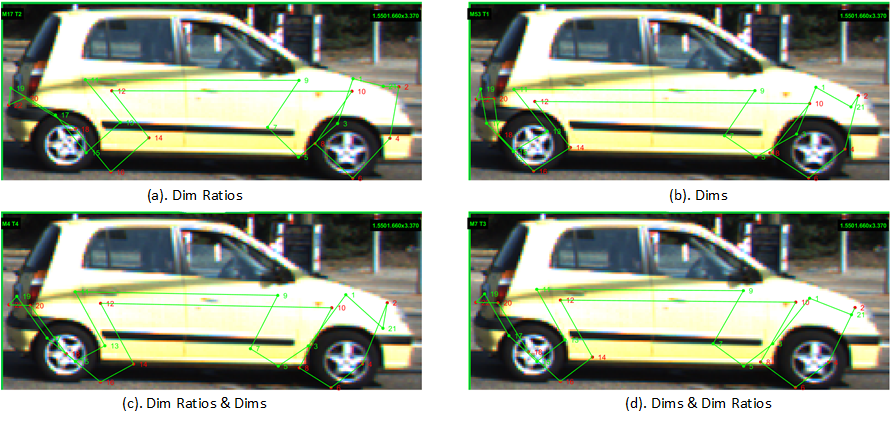
\includegraphics[width=1\textwidth]{model_selection_s.png}
	\caption{One labelled example of four model selection strategies. (a). Dim Ratios. (b). Dims. (c). Dim Ratios \& Dims. (d). Dims \& Dim Ratios. }
	\centering
	\label{figure:model_selection_s}
\end{figure}

\subsubsection{Difficulty Levels For Dataset Division}
KITTI set three levels for 3D object detection based on three factors: the size of the 2D bounding boxes, degree of occlusion and truncation. In order to compare the influence brought by these three factors, we extend the division into nine levels, as shown in Table \ref{levels_d}. And Level 4 is used to evaluate other design choices because it is neither too complicate nor too simple.
\tbd [more detailed level to check the difficulty of each property]

\renewcommand{\arraystretch}{1.0}
\begin{table}[H]
	\centering
	\caption{Levels of difficulty. Level 2, 6, and 8 corresponds to the Easy, Moderate, and Hard defined by KITTI \cite{Geiger2012CVPR}.}
	\label{levels_d}
	\resizebox{\textwidth}{!}{
	\begin{tabular}{|c|c|c|c|}
		\hline
		Difficulty level       & Min. bounding box height & Max. Occlusion   & Max. Occlusion \\ \hline
		Level 1   & 40 Px  & 0       & 0     \\ \hline
		\textbf{Level 2 (Easy)}     & \textbf{40 Px}  & \textbf{0}       & \textbf{15\%}  \\ \hline
		Level 3   & 40 Px  & 0, 1    & 15\%  \\ \hline
		Level 4   & 40 Px  & 0, 1    & 30\%  \\ \hline
		Level 5   & 32 Px  & 0, 1    & 30\%  \\ \hline
		\textbf{Level 6 (Moderate)} & \textbf{25 Px}  & \textbf{0, 1}    & \textbf{30\%}  \\ \hline
		Level 7   & 25 Px  & 0, 1, 2 & 30\%  \\ \hline
		\textbf{Level 8 (Hard)}     & \textbf{25 Px}  & \textbf{0, 1, 2} & \textbf{50\%}  \\ \hline
		Level 9   & 25 Px  & 0, 1, 2, 3       & 70\%  \\ \hline
	\end{tabular}
}
\end{table}

We train the network for these nine levels to their best with the identical foundation and the results of six tasks are shown in Table \ref{levels_p}. \tbd further analysis ref. to papers

% Please add the following required packages to your document preamble:
% \usepackage{graphicx}
\begin{table}[]
	\centering
	\caption{Performance of six tasks at different difficult levels.}
	\label{levels_p}
	\resizebox{\textwidth}{!}{%
		\begin{tabular}{|c|c|c|c|c|c|c|}
			\hline
			& \begin{tabular}[c]{@{}c@{}}3D bounding\\ box estimation\end{tabular} & \begin{tabular}[c]{@{}c@{}}3D localization\\ ($Loc. < 1m$)\end{tabular} & \begin{tabular}[c]{@{}c@{}}3D orientation\\ estimation\end{tabular} & \begin{tabular}[c]{@{}c@{}}3D dimension\\ estimation\end{tabular} & \begin{tabular}[c]{@{}c@{}}2D part\\ localization\end{tabular} & \begin{tabular}[c]{@{}c@{}}2D part\\ visibility\end{tabular} \\ \hline
			Level 1 & \textbf{33.54} & 65.97 & \textbf{99.77} & 99.63 & \textbf{99.78} & \textbf{98.03} \\ \hline
			Level 2 & 34.00 & \textbf{67.77} & 99.76 & 99.76 & 99.32 & 97.77 \\ \hline
			Level 3 & 32.49 & 66.81 & 98.96 & \textbf{99.79} & 98.91 & 95.50 \\ \hline
			Level 4 & 30.92 & 65.60 & 99.01 & 99.73 & 98.72 & 94.65 \\ \hline
			Level 5 & 29.41 & 59.91 & 98.67 & 99.73 & 98.65 & 94.53 \\ \hline
			Level 6 & 26.68 & 57.16 & 98.55 & 99.60 & 98.90 & 94.92 \\ \hline
			Level 7 & 24.10 & 52.70 & 97.83 & 99.54 & 98.48 & 94.24 \\ \hline
			Level 8 & 22.86 & 51.35 & 97.30 & 99.48 & 97.52 & 93.92 \\ \hline
			Level 9 & 20.05 & 47.75 & 96.78 & 99.21 & 96.05 & 92.59 \\ \hline
		\end{tabular}%
	}
\end{table}

\subsubsection{Cost Function}

We have described the loss function we used in Section \ref{loss_functions} and here we give reasons for our choices.

The categorical cross entropy loss is the standard choice for multi-class classification but for regression, there are plenty of choices. We select out and do experiment on the following loss functions:  mean squared error \cite{4775883}, mean absolute error \cite{2005ClRes3079W}, Huber loss \cite{huber1964}, Charbonnier loss \cite{413553},  a robust smooth $L_1$ loss function defined in \cite{DBLP:journals/corr/Girshick15}, and our modified smooth $L_1$ loss function defined in Section \ref{loss_functions}.

We experiment with these loss functions with the same setup on Level 4 and evaluate their performance on six tasks with the validation data. The results are shown in Table \ref{p_loss_fcn}. Our modified loss for regression tasks (the first five) outperforms all the others and only has a slight impact on the classification task. The main reason for the modification is that we normalize the labels into the range $[1, 1]$ and most of them falls in $[-0.5, 0.5]$. 

\renewcommand{\arraystretch}{1.2}
\begin{table}[H]
	\centering
	\caption{Performance of six tasks with different loss functions.}
	\label{p_loss_fcn}
	\resizebox{\textwidth}{!}{
	\begin{tabular}{|c|c|c|c|c|c|c|}
		\hline
		Loss function & \begin{tabular}[c]{@{}c@{}}3D bounding\\ box estimation\end{tabular} & \begin{tabular}[c]{@{}c@{}}3D localization\\ ($Loc.<1m$)\end{tabular} & \begin{tabular}[c]{@{}c@{}}3D orientation\\ estimation\end{tabular} & \begin{tabular}[c]{@{}c@{}}3D dimension\\ estimation\end{tabular} & \begin{tabular}[c]{@{}c@{}}2D part \\ localization\end{tabular} & \begin{tabular}[c]{@{}c@{}}2D part\\ visibility\end{tabular} \\ \hline
		\begin{tabular}[c]{@{}c@{}}Charbonnier loss\\ $\epsilon$=0.01\end{tabular} & 28.94 & 58.57 & 98.30 & 99.59 & 98.09 & 93.95 \\ \hline
		\begin{tabular}[c]{@{}c@{}}Charbonnier loss\\ $\epsilon$=0.0001\end{tabular} & 27.3 & 59.04 & 97.89 & \textbf{99.73} & 97.7 & 92.27 \\ \hline
		\begin{tabular}[c]{@{}c@{}}Huber loss\\ $\delta$=0.5\end{tabular} & 25.87 & 58.77 & 98.42 & 99.59 & 98.06 & 94.54 \\ \hline
		mean absolute error & 4.3 & 17.54 & 90.02 & 92.42 & 86.59 & 93.24 \\ \hline
		mean squared error & 7.51 & 25.94 & 94.02 & 97.61 & 88.81 & 93.48 \\ \hline
		robust smooth $L_1$ & 26.21 & 61.09 & 98.47 & 99.66 & 98.11 & \textbf{94.66} \\ \hline
		modified smooth $L_1$ & \textbf{27.39} & \textbf{62.59} & \textbf{98.67} & \textbf{99.73} & \textbf{98.3} & 94.45 \\ \hline
	\end{tabular}%
}
\end{table}

Based on the experiment above, we tune the loss weights: $\lambda_{coord}$, $\lambda_{temp}$ and $\lambda_{visib}$, defined in Eq \ref{eq12}. As mentioned in Section \ref{normalization}, we have normalized the magnitude of all labels into the same range $[-1, 1]$. This label normalization alleviates the difficulties of loss weights tuning because we can focus on the importance of tasks without paying special attention to their quantities.


We apply grid search to find the optimal loss weight combination which results in best performance on the six tasks. Grid search is a common but sometimes expensive practice \cite{Goodfellow-et-al-2016} but the time to train our network is acceptable because we use pre-trained models to initialize our network, . The $\lambda_{visib}$ is assigned 1, $\lambda_{coord}$ and $\lambda_{temp}$ are chosen from the set $\{1, 3, 10, 30\}$ because 2D coordinates and template proximity is much more important than visibility for 3D object detection. The results are shown in Table \ref{p_lw}. The $(\lambda_{coord}=10$, $\lambda_{temp}=1)$ combination is optimal among all choices \ie it performs better on four tasks and only slightly worse on the other two tasks than other weights combinations. This is because the 2D coordinates are used to perform 2D-3D matching and a small deviation of one points in image can lead to a large difference in the world coordinate system. Besides, the template proximity can't diverge too much due to the matching strategy where the a big deviation only happens when all the predicted dimension ratios vectors are ridiculously wrong.


\renewcommand{\arraystretch}{1.2}
\begin{table}[H]
	\centering
	\caption{Performance of six tasks with different loss weights combinations.}
	\label{p_lw}
	\resizebox{\textwidth}{!}{%
		\begin{tabular}{|c|c|c|c|c|c|c|}
			\hline
			($\lambda_{coord}$, $\lambda_{temp}$) & \begin{tabular}[c]{@{}c@{}}3D bounding\\ box estimation\end{tabular} & \begin{tabular}[c]{@{}c@{}}3D localization\\ ($Loc.<1m$)\end{tabular} & \begin{tabular}[c]{@{}c@{}}3D orientation\\ estimation\end{tabular} & \begin{tabular}[c]{@{}c@{}}3D dimension\\ estimation\end{tabular} & \begin{tabular}[c]{@{}c@{}}2D part\\ localization\end{tabular} & \begin{tabular}[c]{@{}c@{}}2D part\\ visibility\end{tabular} \\ \hline
			(1, 1) & 29.35 & 63.89 & 98.53 & 99.66 & 98.39 & 94.98 \\ \hline
			(1, 3) & 25.19 & 56.93 & 97.87 & 99.59 & 97.7 & 94.18 \\ \hline
			(1, 10) & 24.71 & 53.65 & 98.05 & 99.66 & 97.61 & 94.41 \\ \hline
			(1, 30) & 19.59 & 45.39 & 97.68 & 99.59 & 96.46 & 93.92 \\ \hline
			(3, 1) & 29.28 & 61.84 & 98.78 & 99.59 & 98.56 & 94.71 \\ \hline
			(3, 3) & 29.76 & 63.89 & 98.63 & 99.66 & 98.55 & 94.72 \\ \hline
			(3, 10) & 25.67 & 58.7 & 98.04 & 99.52 & 97.56 & 94.28 \\ \hline
			(3, 30) & 21.98 & 49.69 & 98.32 & 99.59 & 97.18 & 93.99 \\ \hline
			(10, 1) & \textbf{34.06} & \textbf{68.46} & 99.16 & 99.66 & \textbf{98.98} & \textbf{95.18} \\ \hline
			(10, 3) & 30.58 & 63.41 & 98.71 & \textbf{99.73} & 98.61 & 94.38 \\ \hline
			(10, 10) & 32.7 & 66.28 & 98.60 & 99.59 & 98.62 & 94.52 \\ \hline
			(10, 30) & 27.03 & 60.27 & 98.09 & \textbf{99.73} & 97.79 & 93.96 \\ \hline
			(30, 1) & 33.17 & 66.96 & \textbf{99.24} & 99.66 & 98.95 & 94.91 \\ \hline
			(30, 3) & 31.4 & 66.62 & 98.87 & \textbf{99.73} & 98.88 & 94.43 \\ \hline
			(30, 10) & 31.74 & 68.12 & 98.69 & 99.66 & 98.61 & 94.46 \\ \hline
			(30, 30) & 31.19 & 65.32 & 98.66 & 99.52 & 98.36 & 93.43 \\ \hline
		\end{tabular}%
	}
\end{table}


\subsubsection{Learning Rate and Weight Decay}

Learning rate is one hyperparameter that determines how much the parameters of the network are updated with respect to the gradients of the cost function. It is perhaps the most crucial hyperparameter because it plays a more complicated and important role in affecting the effective capability of the model than the others. There is a typical U-shaped relationship between the learning rate and the model's performance. If it is too small, the training is more stable but the time to train the model is much longer and sometimes, the training might get stuck on a plateau region or around a saddle point. On the other hand, if it is too large, the training can converge more quickly but is more variable because it may fail to converge or even diverge. Only a proper learning rate can achieve the best performance of the model. Therefore as Goodfellow \etal suggest that if you can only tune one hyperparameter, tune the learning rate \cite{Goodfellow-et-al-2016}.

Automatic learning rate selection methods alleviate the difficulty hugely, but they are too computational expensive so that we manually tune it. We first apply a "LR range test" \cite{DBLP:journals/corr/Smith15a}, training the network for several epochs with the learning rate increasing linearly in a guessing range and then analysing the loss over these learning rates. From the test result in Figure \ref{figure:lr_test}, the correct learning falls in the range $[10^{-6}, 10^{-3}]$. 

\begin{figure}[H]		
	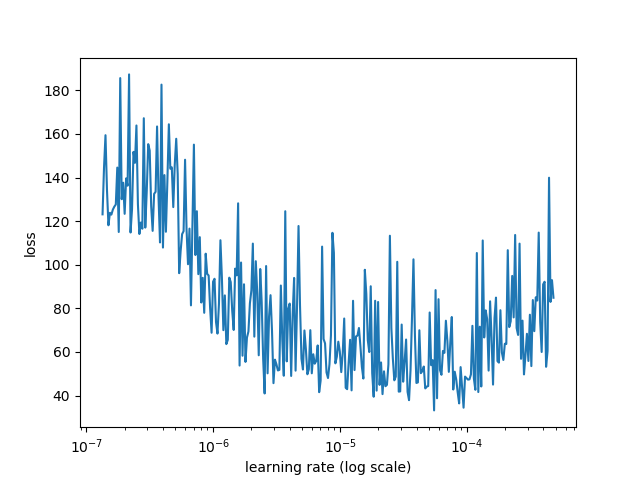
\includegraphics[width=0.8\textwidth]{LR_range_test.png}
	\caption{Results of "LR range test": loss over monotonically increasing learning rate. }
	\centering
	\label{figure:lr_test}
\end{figure}

Weight decay is a regularization technique which is used to prevent the weights of the model getting too big as to be overfitting. Since Keras Optimizers \cite{chollet2015keras} take both learning rate and weight decay as input parameters, we apply grid search for both of them together. The results are shown in Table \ref{lrd}. The combination of $(10^{-5}, 10^{-6})$ for learning rate and weight decay respectively achieves the best performance except for 2D part visibility classification with $0.2\%$ lower. Therefore we select this combination. The best results in Table \ref{lrd} is worse than in Table \ref{p_lw} because we set all loss weights as 1 here so that they are close to the results in first row of Table \ref{p_lw}. \tbd wait for new results of lr5 \& lr6

% Please add the following required packages to your document preamble:
% \usepackage{graphicx}
\begin{table}[]
	\centering
	\caption{Performance of six tasks with different learning rate and weight decay combinations}
	\label{lrd}
	\resizebox{\textwidth}{!}{%
		\begin{tabular}{|c|c|c|c|c|c|c|}
			\hline
			\begin{tabular}[c]{@{}c@{}}(learning rate, \\weight decay)\end{tabular} & \begin{tabular}[c]{@{}c@{}}3D bounding\\ box estimation\end{tabular} & \begin{tabular}[c]{@{}c@{}}3D localization\\ ($Loc.<1m$)\end{tabular} & \begin{tabular}[c]{@{}c@{}}3D orientation\\ estimation\end{tabular} & \begin{tabular}[c]{@{}c@{}}3D dimension\\ estimation\end{tabular} & \begin{tabular}[c]{@{}c@{}}2D part\\ localization\end{tabular} & \begin{tabular}[c]{@{}c@{}}2D part\\ visibility\end{tabular} \\ \hline
			$(10^{-4}, 10^{-4})$ & 0.491 & 0.564 & 0.977 & \textbf{0.997} & 0.981 & 0.948 \\ \hline
			$(10^{-4}, 10^{-5})$ & 0.54 & 0.608 & 0.98 & 0.996 & 0.983 & \textbf{0.951} \\ \hline
			$(10^{-4}, 10^{-6})$ & 0.499 & 0.566 & 0.978 & \textbf{0.997} & 0.984 & \textbf{0.951} \\ \hline
			$(10^{-4}, 10^{-7})$ & 0.522 & 0.595 & 0.979 & \textbf{0.997} & 0.982 & 0.95 \\ \hline
			$(10^{-5}, 10^{-4})$ & 0.519 & 0.596 & 0.979 & 0.994 & 0.975 & 0.932 \\ \hline
			$(10^{-5}, 10^{-5})$ & 0.552 & 0.625 & 0.985 & 0.995 & 0.981 & 0.941 \\ \hline
			$(10^{-5}, 10^{-6})$ & \textbf{0.539} & \textbf{0.631} & \textbf{0.986} & \textbf{0.997} & \textbf{0.986} & 0.949 \\ \hline
			$(10^{-5}, 10^{-7})$ & 0.538 & 0.627 & 0.984 & \textbf{0.997} & 0.983 & 0.946 \\ \hline
			$(10^{-6}, 10^{-4})$ & 0.382 & 0.442 & 0.962 & 0.99 & 0.951 & 0.892 \\ \hline
			$(10^{-6}, 10^{-5})$ & 0.405 & 0.479 & 0.971 & 0.99 & 0.958 & 0.905 \\ \hline
			$(10^{-6}, 10^{-6})$ & 0.38 & 0.46 & 0.969 & 0.988 & 0.952 & 0.897 \\ \hline
			$(10^{-6}, 10^{-7})$ & 0.392 & 0.474 & 0.969 & 0.99 & 0.955 & 0.901 \\ \hline
		\end{tabular}%
	}
\end{table}

\subsubsection{Feature Extractor}
Our baseline network uses ResNet50 as feature extractor. But there are several other out-of-shelf network with pre-trained weights so that we carry out experiments on them. The other base nets we choose are VGG16, VGG19 \cite{DBLP:SimonyanZ14a}, InceptionV3 \cite{DBLP:journals/corr/SzegedyVISW15}, Xception \cite{DBLP:journals/corr/Chollet16a}, DenseNet121, DenseNet169, DenseNet201\cite{DBLP:journals/corr/HuangLW16a}.

As before, we train all the models with different base nets on the same setup with data Level 4. Their performance on six tasks are shown in Table \ref{basenets}. According to their performance, only VGG19 can perform better than ResNet50 on the whole. Therefore, we includes VGG19 for our final evaluation in Section \ref{exp_res}.

\tbd [is it necessary to analyse why they perform this way]

\begin{table}[H]
	\centering
	\caption{Performance of six tasks with different base net.}
	\label{basenets}
	\resizebox{\textwidth}{!}{%
		\begin{tabular}{|c|c|c|c|c|c|c|}
			\hline
			Base Net & \begin{tabular}[c]{@{}c@{}}3D bounding\\ box estimation\end{tabular} & \begin{tabular}[c]{@{}c@{}}3D localization\\ ($Loc.<1m$)\end{tabular} & \begin{tabular}[c]{@{}c@{}}3D orientation\\ estimation\end{tabular} & \begin{tabular}[c]{@{}c@{}}3D dimension\\ estimation\end{tabular} & \begin{tabular}[c]{@{}c@{}}2D part\\ localization\end{tabular} & \begin{tabular}[c]{@{}c@{}}2D part\\ visibility\end{tabular} \\ \hline
			ResNet50 & \textbf{30.85} & \textbf{64.98} & \textbf{99.03} & 99.73 & \textbf{98.77} & 94.74 \\ \hline
			VGG16 & 29.22 & 57.82 & 98.54 & \textbf{99.86} & 98.44 & \textbf{95.76} \\ \hline
			VGG19 & \textbf{31.54} & 64.23 & \textbf{99.22} & \textbf{99.93} & \textbf{98.68} & \textbf{96.05} \\ \hline
			InceptionV3 & 27.51 & 63.07 & 97.90 & 99.25 & 97.82 & 93.83 \\ \hline
			Xception & 21.09 & 49.83 & 96.05 & 98.91 & 95.22 & 89.17 \\ \hline
			DenseNet121 & 26.28 & 59.73 & 98.15 & 99.52 & 97.47 & 93.26 \\ \hline
			DenseNet169 & 30.24 & \textbf{65.05} & 98.27 & 99.59 & 98.05 & 93.8 \\ \hline
			DenseNet201 & 27.3 & 61.37 & 98.69 & 99.59 & 98.08 & 93.45 \\ \hline
		\end{tabular}%
	}
\end{table}

\subsubsection{Selection of Characteristic Points}

The number of characteristic points is another factor that influences the performance. Theoretically, the more points the better accuracy of 2D-3D matching because it is more robust to outliers. The outliers are eliminated via RANSAC \cite{Fischler:1981:RSC:358669.358692}. But the labelling of these points is time-consuming and demanding. Moreover, the exact locations of points also affect the performance, too. Some points may be hard to detect correctly with the network due to their context in the image and some even distribute differently among various shapes of vehicles. 

\begin{figure}[ht]		
	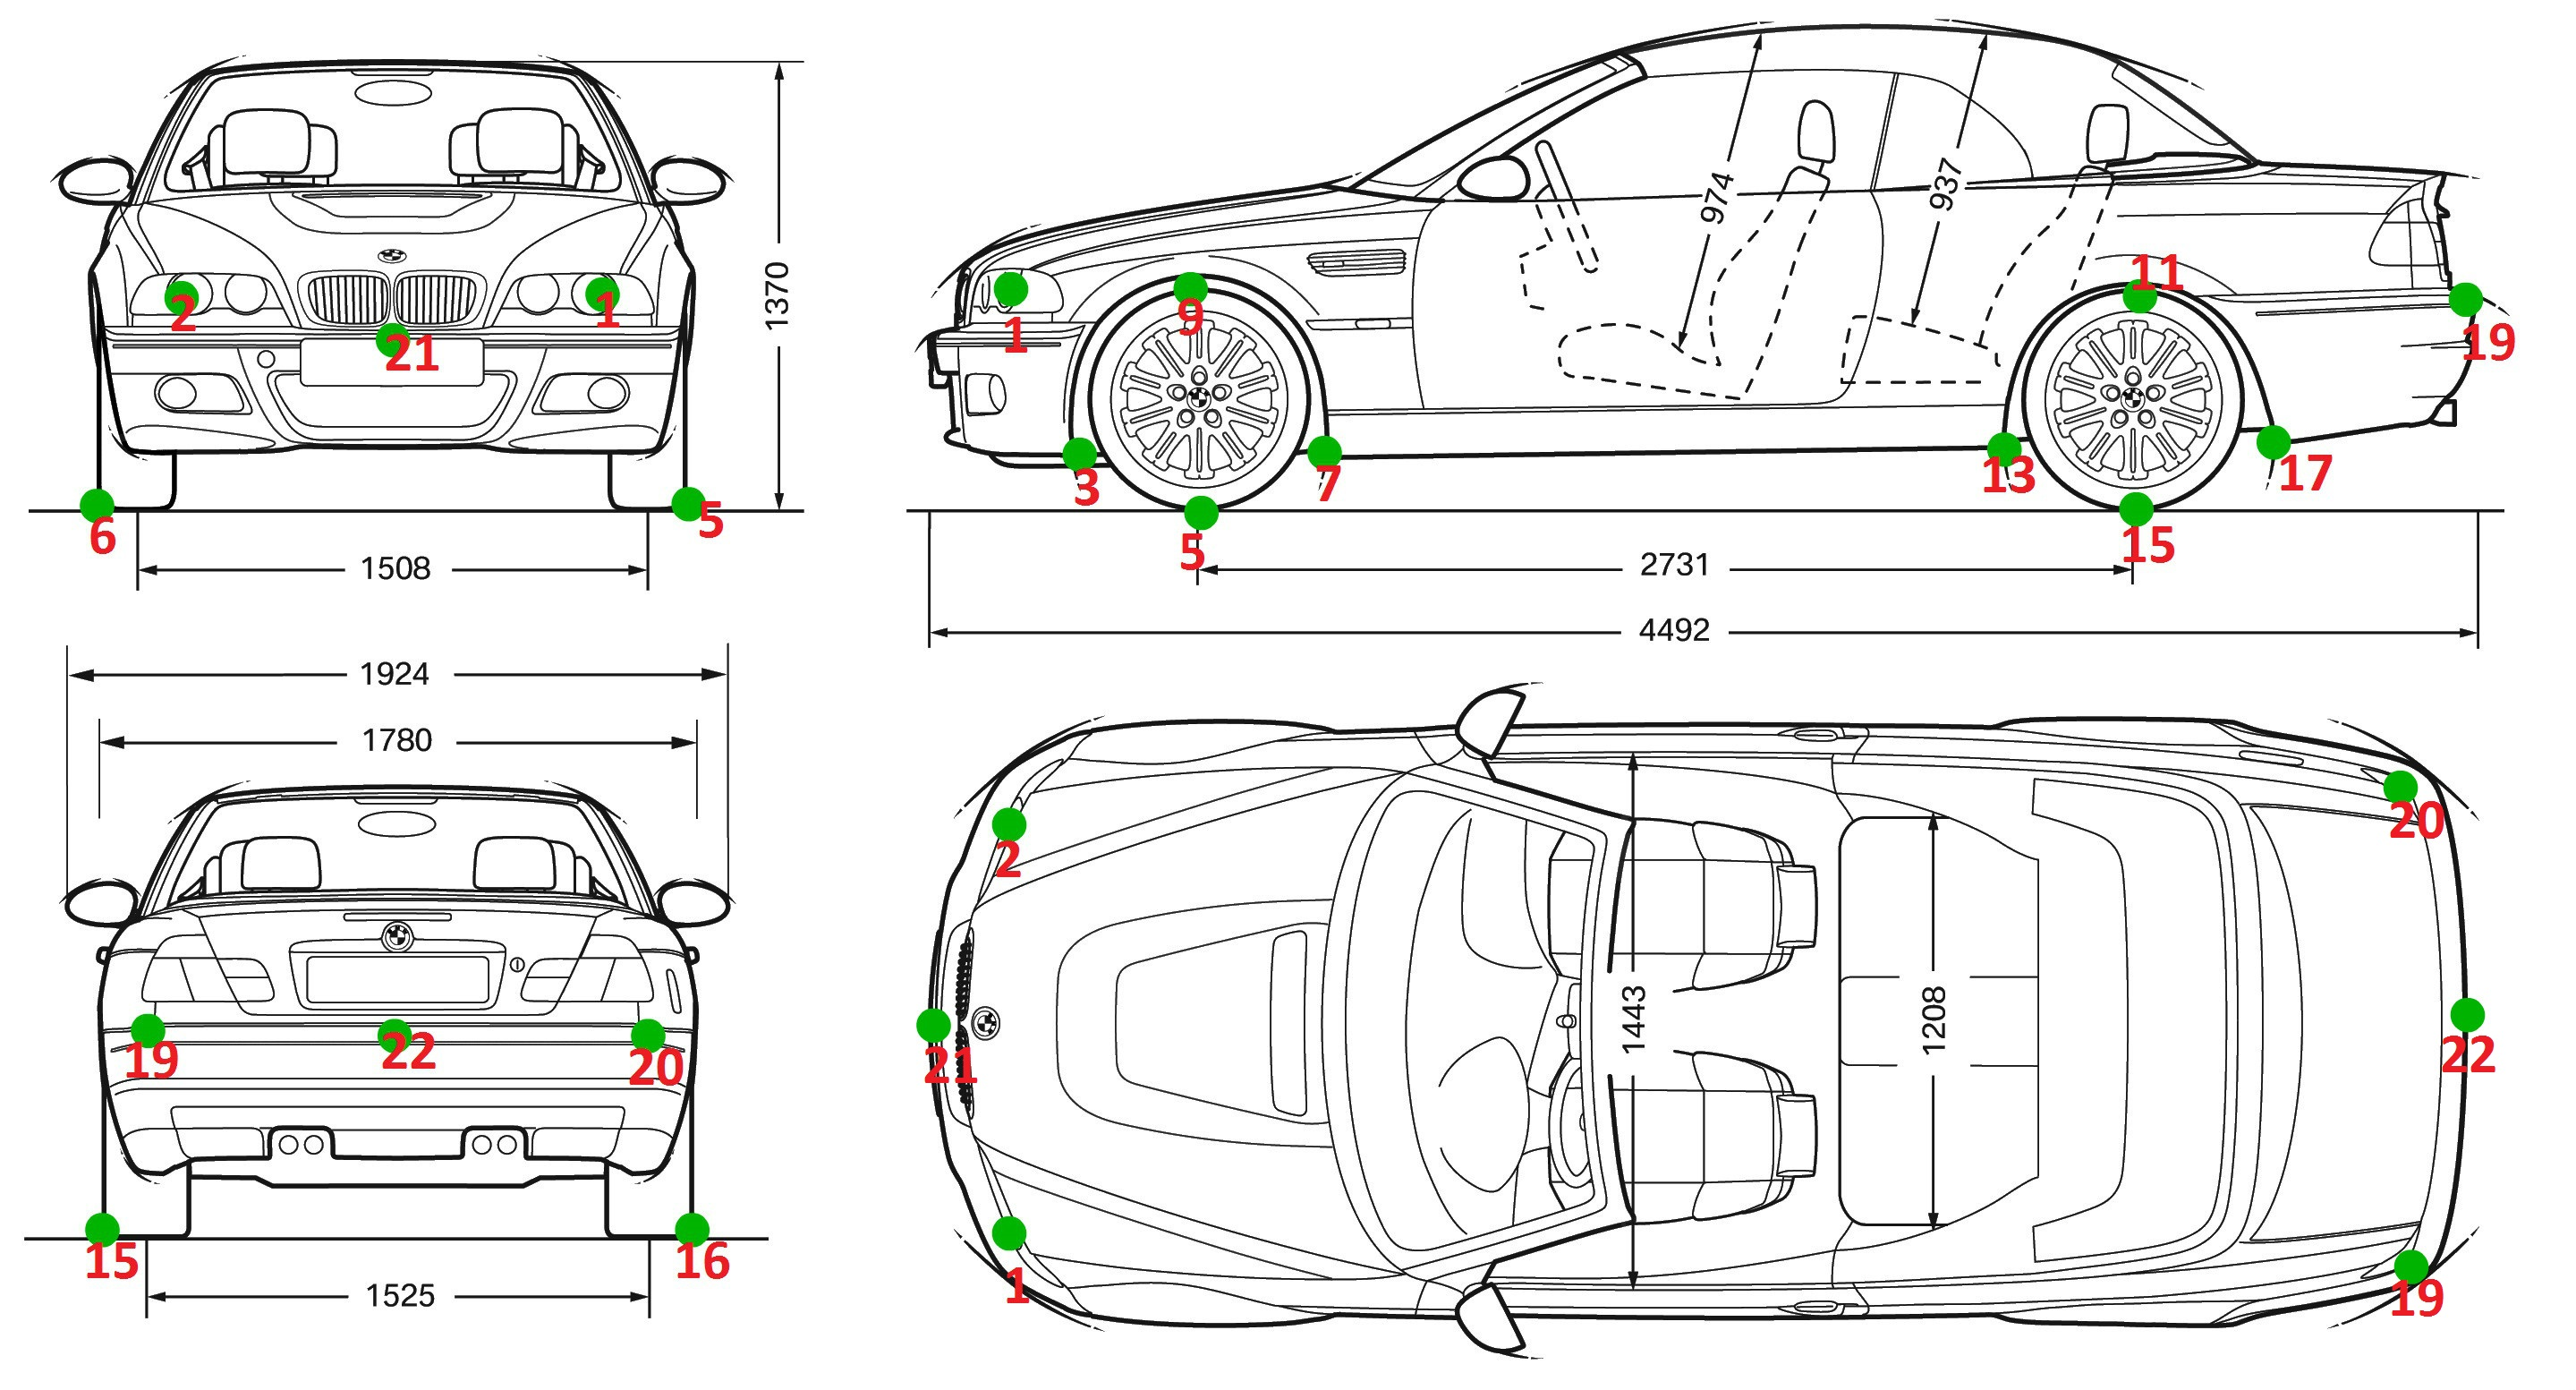
\includegraphics[width=1\textwidth]{point_notation_22.jpg}
	\caption{The schematic diagram for 22 characteristic points. point 1 and 2 denotes the center of two headlights; point 3-18 are around four wheels; point 19 and 20 denote two rear corners; and point 21 and 22 denotes the frontmost and  backmost points along the ordinate axis of the vehicle.}
	\centering
	\label{figure:point_notation_22}
\end{figure}

As the Figure \ref{figure:point_notation_22} shows, we initially label 22 points for each model to construct its corresponding 3D sketch. The points around four wheels are most important because their geometric characters are most stable and rigid, and usually, half of them are visible if not occluded by other objects. However, points 1, 2, 19, and 20 around the front and rear may vary a lot with respect to different shape of the vehicles. We still consider them because they have clear semantic meaning and we may need these points when the points around wheels are not visible, \eg when the vehicle is following another vehicle on the straight lane. The geometric property of point 21 and 22 are stable but their context is not as clear as the points around the wheels.

Therefore we do some experiment on the selection of these points. We select three cases: 1). 16 points: points 3-18; 2). 20 points: points 1-18 and points 21-22; 3). 22 points: point 1-22. We train these three case on data Level 2, 6, and 8 which corresponds to the easy, moderate, and hard defined by KITTI. The reason for training on three levels instead of only Level 4 as before is that the size of the 2D bounding box and degree of the occlusion and truncation impact the geometric appearance of vehicles in images and thus affect detection of these points.

The experiment results are shown in Table \ref{point_selection}.  According to the results, 22-point case works best when the input patch is relatively bigger, \ie the minimal height for a 2D bounding box is 40 pixels. This is because when the vehicles are large in image, it is easier to estimate the 2D coordinates and the template proximity and in this scenario, the more the points, the better the performance. However, when very small vehicles are taken into consideration, it become harder to predict the 2D coordinates correctly because these key points in a small vehicle locate very close to each other. 

\tbd [it requires more results to render the reasons. therefore i train them in 9 levels and then to evaluate the res.]



% Please add the following required packages to your document preamble:
% \usepackage{graphicx}
\begin{table}[H]
	\centering
	\caption{The performance of six tasks with different data difficulty level and different point selection cases.}
	\label{point_selection}
	\resizebox{\textwidth}{!}{%
		\begin{tabular}{|c|c|c|c|c|c|c|}
			\hline
			& \begin{tabular}[c]{@{}c@{}}3D bounding\\ box estimation\end{tabular} & \begin{tabular}[c]{@{}c@{}}3D localization\\ ($Loc.< 1m$)\end{tabular} & \begin{tabular}[c]{@{}c@{}}3D orientation\\ estimation\end{tabular} & \begin{tabular}[c]{@{}c@{}}3D dimension\\ estimation\end{tabular} & \begin{tabular}[c]{@{}c@{}}2D part\\ localization\end{tabular} & \begin{tabular}[c]{@{}c@{}}2D part\\ visibility\end{tabular} \\ \hline
			Easy\_P16 & 31.28 & 64.81 & 99.75 & \textbf{99.88} & \textbf{99.48} & \textbf{97.82} \\ \hline
			Easy\_P20 & 34.00 & 67.77 & \textbf{99.76} & 99.76 & 99.32 & 97.77 \\ \hline
			Easy\_P22 & \textbf{34.83} & \textbf{69.43} & 99.16 & 99.76 & 99.35 & 97.73 \\ \hline
			\multicolumn{7}{|c|}{} \\ \hline
			Moderate\_P16 & 25.39 & 56.22 & \textbf{99.05} & \textbf{99.64} & 98.88 & 94.98 \\ \hline
			Moderate\_P20 & 26.68 & 57.16 & 98.55 & 99.60 & \textbf{98.90} & 94.92 \\ \hline
			Moderate\_P22 & \textbf{28.16} & \textbf{57.21} & 98.86 & \textbf{99.64} & 98.89 & \textbf{95.02} \\ \hline
			\multicolumn{7}{|c|}{} \\ \hline
			Hard\_P16 & \textbf{25.04} & \textbf{53.39} & \textbf{98.53} & \textbf{99.55} & \textbf{98.28} & \textbf{94.15} \\ \hline
			Hard\_P20 & 22.86 & 51.35 & 97.30 & 99.48 & 97.52 & 93.92 \\ \hline
			Hard\_P22 & 23.12 & 50.63 & 97.63 & 99.35 & 98.01 & 94.00 \\ \hline
		\end{tabular}%
	}
\end{table}


